% 2011 年山东卷理科第 19 题：多面体 ABCD-EFG，AB = 2EF，EF∥AB，FG∥BC，EG∥AC，EA⊥平面 ABCD。
% 来源 PDF：普通高考/2011/2011山东理.pdf，SHA-256 d0f409fd3fa82b12c210d587c8412d4c446946a201f87d124e2fc17c5a50db16。
% 原页：第 2 页（A3 三栏）第 1 栏上部，书页码 690。
% 重绘依据：照原页作斜二测示意（AC = BC = 2AE）。经核实该多面体共有 7 个面：
%   底面 ABCD（平行四边形），面 ABFE（等腰梯形，AB∥EF 且 AB=2EF），面 ADE（三角形），
%   面 BCFG（四边形，FG∥BC），面 CDG（三角形），面 DEG（三角形），面 EFG（三角形）。
%   可见棱（实线）：BC、CD、CG、DE、DG、EF、EG、FB、FG；
%   被遮棱（虚线）：AB、AD、AE；另按原页用虚线画出底面对角线 AC（标出 ∠ACB=90°）与线段 GM（M 为 AD 中点）。
%   拓扑与原页一致，不按比例。
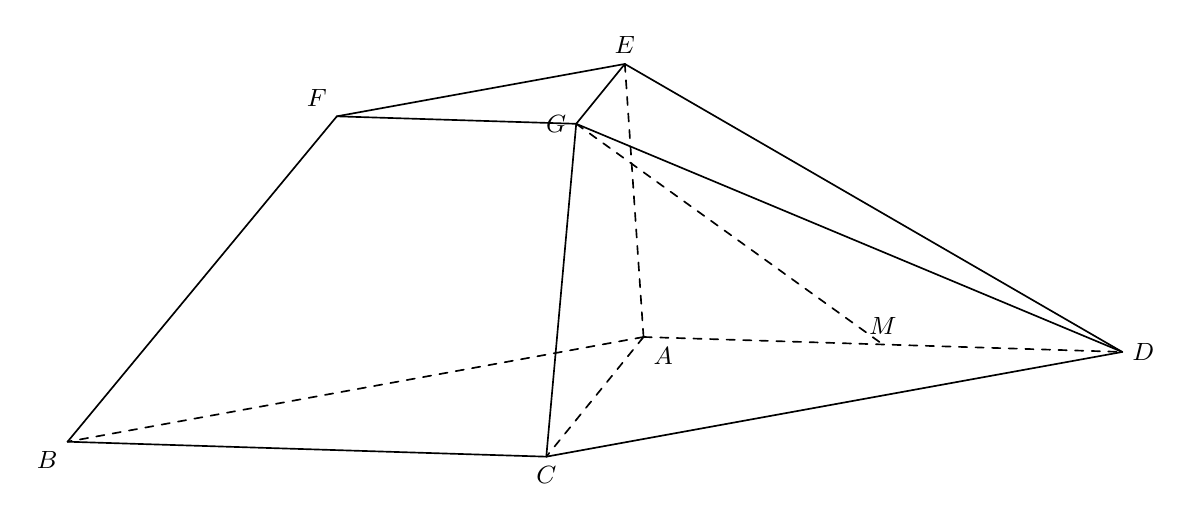
\begin{tikzpicture}[scale=0.95, >=stealth, semithick, font=\small,
  line cap=round]
  \coordinate (B) at (3.60,4.50);
  \coordinate (C) at (10.00,4.30);
  \coordinate (A) at (11.30,5.90);
  \coordinate (D) at (17.70,5.70);
  \coordinate (E) at (11.05,9.55);
  \coordinate (F) at (7.20,8.85);
  \coordinate (G) at (10.40,8.75);
  \coordinate (M) at (14.50,5.80);
  % 可见棱
  \draw (B) -- (C) -- (D);
  \draw (C) -- (G);
  \draw (D) -- (E);
  \draw (D) -- (G);
  \draw (E) -- (F);
  \draw (E) -- (G);
  \draw (F) -- (B);
  \draw (F) -- (G);
  % 被遮棱
  \draw[dashed] (A) -- (B);
  \draw[dashed] (A) -- (D);
  \draw[dashed] (A) -- (E);
  % 底面对角线 AC（原页用虚线画出，以显示 ∠ACB = 90°）
  \draw[dashed] (A) -- (C);
  % 线段 GM（M 为 AD 的中点）
  \draw[dashed] (G) -- (M);
  % 顶点标注
  \node[above] at (E) {$E$};
  \node[above left] at (F) {$F$};
  \node[left] at (G) {$G$};
  \node[below left] at (B) {$B$};
  \node[below] at (C) {$C$};
  \node[below right] at (A) {$A$};
  \node[right] at (D) {$D$};
  \node[above] at (M) {$M$};
\end{tikzpicture}
